\documentclass{article}
% Chinese
% \documentclass[UTF8, nofonts, mathptmx, 12pt, onecolumn]{article}
% \usepackage{xeCJK}
% \setCJKmainfont{SimSun}
\usepackage{amsmath}
\usepackage{amsfonts}
\usepackage{amssymb}
\usepackage{wasysym}
% \usepackage{ctex}
\usepackage{graphicx}
\usepackage{float}
\usepackage{geometry}
\geometry{a4paper,scale=0.8}
\usepackage{caption}
\usepackage{subcaption}
% \newcommand{\oiint}{\mathop{{\int\!\!\!\!\!\int}\mkern-21mu \bigcirc} {}}
\newcommand*{\dif}{\mathop{}\!\mathrm{d}}
\newcommand*{\md}{\mathop{}\!\mathrm{d}}
\newcommand*{\me}{\mathrm{e}}

\usepackage{parskip}
\setlength{\parindent}{0cm}

\usepackage{bm}
\let\Oldmathbf\mathbf
\renewcommand{\mathbf}[1]{\boldsymbol{\Oldmathbf{#1}}}
\let\eqnarray\align

\author{Xiping Hu}
\usepackage{authblk}
\author{Xiping Hu}
\affil{https://hxp.plus/}
\title{Homework for Chapter 3}

\begin{document}
\maketitle

\begin{figure}[H]
  \centering
  
\includegraphics[width=\linewidth]{figures/1}
  \label{fig:}
\end{figure}

\begin{equation*}
  \begin{aligned}
    E= \dfrac{hc}{\lambda}  = 1.98645 \times 10^{-15} \  \mathrm{J \cdot m}
  \end{aligned}
\end{equation*}

\begin{equation*}
  \begin{aligned}
    p = \dfrac{h}{\lambda} =  6.62607 \times 10^{-24} \ \mathrm{J \cdot s}
  \end{aligned}
\end{equation*}

\begin{figure}[H]
  \centering
  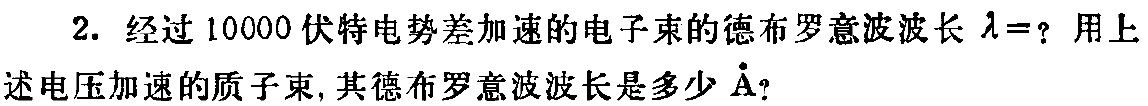
\includegraphics[width=\linewidth]{figures/2}
  \label{fig:}
\end{figure}

\begin{equation*}
  \begin{aligned}
    v = \sqrt{\dfrac{2 E_k}{m_0} } = 5.93097 \times 10^7 \  \mathrm{m/s}
  \end{aligned}
\end{equation*}
\begin{equation*}
  \begin{aligned}
    \lambda = \dfrac{h}{m_0 v} = 1.22643 \times 10^{-11} \  \mathrm{m} 
  \end{aligned}
\end{equation*}

\begin{figure}[H]
  \centering
  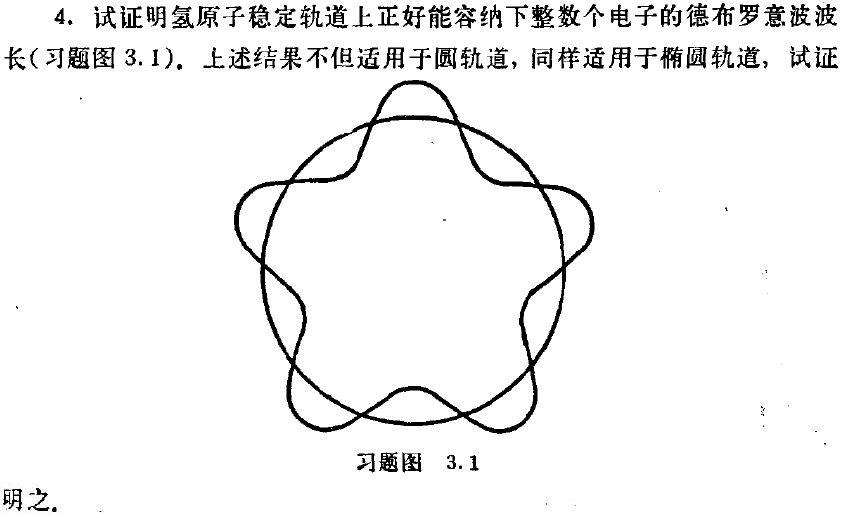
\includegraphics[width=\linewidth]{figures/4}
  \label{fig:}
\end{figure}

In round orbits

\begin{equation*}
  \begin{aligned}
    \oint p_r \md q_r = n_r h \\
    \oint p_\phi \md q_\phi = n_\phi h
  \end{aligned}
\end{equation*}

Since $p_r = 0$

\begin{equation*}
  \begin{aligned}
    \oint m r^2 \dot{\phi} \md \phi = n_\phi h
  \end{aligned}
\end{equation*}
\begin{equation*}
  \begin{aligned}
    2 \pi m v r = n_{\phi} h
  \end{aligned}
\end{equation*}

\begin{equation*}
  \begin{aligned}
    2 \pi r = n_{\phi} \dfrac{h}{m v} 
  \end{aligned}
\end{equation*}

The wave length of the electron is

\begin{equation*}
  \begin{aligned}
    \lambda = \dfrac{h}{p} = \dfrac{h}{m v}  
  \end{aligned}
\end{equation*}

So that

\begin{equation*}
  \begin{aligned}
    2 \pi r = n_{\phi} \lambda
  \end{aligned}
\end{equation*}

When the orbit is shaped in eclipse

\begin{equation*}
  \begin{aligned}
    \oint p_r \md q_r = n_r h \\
    \oint p_\phi \md q_\phi = n_\phi h
  \end{aligned}
\end{equation*}

So that

\begin{equation*}
  \begin{aligned}
    \oint \left( p_r \md r + p_{\phi} \md \phi \right) = n h
  \end{aligned}
\end{equation*}

\begin{equation*}
  \begin{aligned}
    \oint \left( m \dot{r} \md r + m r^2 \dot{\phi} \md \phi \right) = n h
  \end{aligned}
\end{equation*}

\begin{equation*}
  \begin{aligned}
    \oint \left( m \dot{r}^2 \md t + m r^2 \dot{\phi}^2 \md t \right) = n h
  \end{aligned}
\end{equation*}

\begin{equation*}
  \begin{aligned}
    \oint \left[ m \left( \dot{r}^2 + m r^2 \dot{\phi}^2 \right) \right] \md t = n h
  \end{aligned}
\end{equation*}

\begin{equation*}
  \begin{aligned}
    \oint \left[ m v^2 \right] \md t = n h
  \end{aligned}
\end{equation*}

\begin{equation*}
  \begin{aligned}
    \oint m v \md s = n h
  \end{aligned}
\end{equation*}

\begin{equation*}
  \begin{aligned}
    \oint \dfrac{m v}{h}  \md s = n
  \end{aligned}
\end{equation*}

The wavelength of the electron is

\begin{equation*}
  \begin{aligned}
    \lambda = \dfrac{h}{p} = \dfrac{h}{m v}  
  \end{aligned}
\end{equation*}

insert it into

\begin{equation*}
  \begin{aligned}
    \oint \dfrac{\md s}{\lambda}  = n
  \end{aligned}
\end{equation*}

\begin{equation*}
  \begin{aligned}
    \oint \md s = n \lambda
  \end{aligned}
\end{equation*}

\begin{figure}[H]
  \centering
  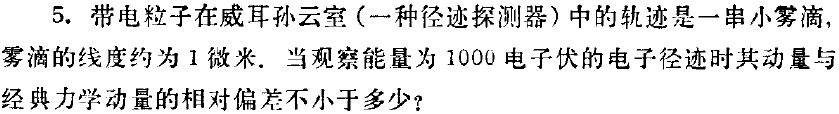
\includegraphics[width=\linewidth]{figures/5}
  \label{fig:}
\end{figure}

\begin{equation*}
  \begin{aligned}
    \Delta p \Delta x \ge \dfrac{\hbar}{2} 
  \end{aligned}
\end{equation*}

\begin{equation*}
  \begin{aligned}
    p = \sqrt{2 m E_k} 
  \end{aligned}
\end{equation*}

\begin{equation*}
  \begin{aligned}
    \dfrac{\Delta p}{p}  = \dfrac{\hbar}{2 \Delta x \sqrt{2 m E_k}} = 3.046 \times 10^{-5}
  \end{aligned}
\end{equation*}

\begin{figure}[H]
  \centering
  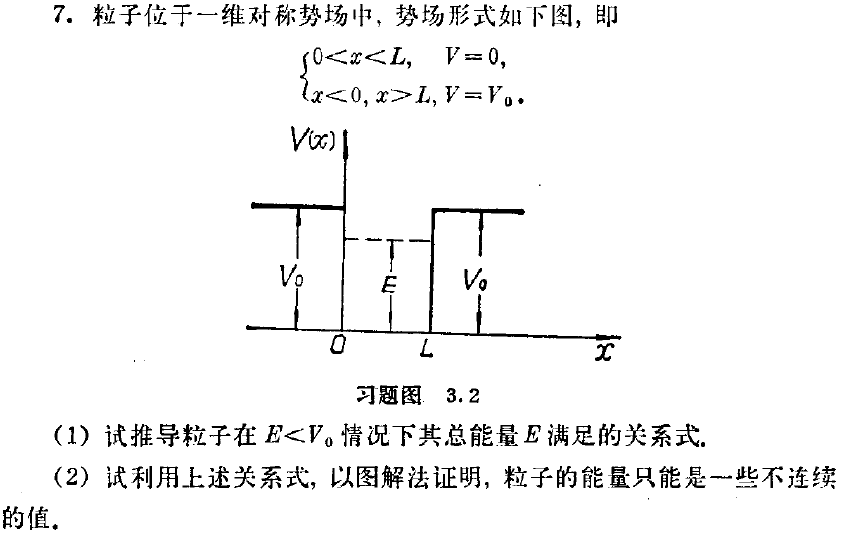
\includegraphics[width=\linewidth]{figures/7}
  \label{fig:}
\end{figure}

\paragraph{Solution for problem (1)}

\begin{equation*}
  \begin{aligned}
    \dfrac{\md^2 \Psi}{\md x^2} + \dfrac{2 m \left( E - V \right)}{\hbar^2} \Psi = 0
  \end{aligned}
\end{equation*}

For $x < 0$

\begin{equation*}
  \begin{aligned}
    \dfrac{\md^2 \Psi}{\md x^2} - \dfrac{2 m \left( V_0 - E \right)}{\hbar^2} \Psi = 0
  \end{aligned}
\end{equation*}

\begin{equation*}
  \begin{aligned}
    \Psi_1 \left( x \right) = A \exp \left[ \sqrt{\dfrac{2 m \left( V_0 - E \right)}{\hbar^2} } x \right]
  \end{aligned}
\end{equation*}

For $0 < x < L$

\begin{equation*}
  \begin{aligned}
     \dfrac{\md^2 \Psi}{\md x^2} + \dfrac{2 m E}{\hbar^2} \Psi = 0   
  \end{aligned}
\end{equation*}

\begin{equation*}
  \begin{aligned}
    \Psi_2 \left( x \right) = B \sin \left[ \sqrt{\dfrac{2 m E}{\hbar^2} } x + \phi \right]
  \end{aligned}
\end{equation*}

For $x > L$

\begin{equation*}
  \begin{aligned}
    \dfrac{\md^2 \Psi}{\md x^2} - \dfrac{2 m \left( V_0 - E \right)}{\hbar^2} \Psi = 0
  \end{aligned}
\end{equation*}

\begin{equation*}
  \begin{aligned}
    \Psi_3 \left( x \right) = C \exp \left[ - \sqrt{\dfrac{2 m \left( V_0 - E \right)}{\hbar^2} } x \right]
  \end{aligned}
\end{equation*}

In conclusion

\begin{equation*}
  \left\{
  \begin{aligned}
    \Psi_1 \left( x \right) &= A \exp \left[ \sqrt{\dfrac{2 m \left( V_0 - E \right)}{\hbar^2} } x \right] = A \exp \left[ \alpha x \right] \\
    \Psi_2 \left( x \right) &= B \sin \left[ \sqrt{\dfrac{2 m E}{\hbar^2} } x + \phi \right] = B \sin \left[ \beta x + \phi \right] \\
    \Psi_3 \left( x \right) &= C \exp \left[ - \sqrt{\dfrac{2 m \left( V_0 - E \right)}{\hbar^2} } x \right] = C \exp \left[ - \alpha x \right]
  \end{aligned}
  \right.
\end{equation*}

By taking logarithms

\begin{equation*}
  \left\{
  \begin{aligned}
    & \log \left[ \Psi_1 \left( x \right) \right] =  \log A + \alpha x \\
    & \log \left[ \Psi_2 \left( x \right) \right]  = \log B  + \log \left[ \sin \left( \beta x + \phi \right) \right] \\
    & \log \left[ \Psi_3 \left( x \right) \right] = \log C - \alpha x
  \end{aligned}
  \right.
\end{equation*}

By taking derivatives

\begin{equation*}
  \left\{
  \begin{aligned}
    & \dfrac{1}{\Psi_1 \left( x \right)} \dfrac{\md \Psi_1 \left( x \right)}{\md x} = \alpha \\
    & \dfrac{1}{\Psi_2 \left( x \right)} \dfrac{\md \Psi_2 \left( x \right)}{\md x} = \beta \cot \left[ \beta x + \phi \right] \\
    & \dfrac{1}{\Psi_3 \left( x \right)} \dfrac{\md \Psi_3 \left( x \right)}{\md x} = - \alpha
  \end{aligned}
  \right.
\end{equation*}

Due to the continuity of $\Psi \left( x \right)$

\begin{equation*}
  \left\{
  \begin{aligned}
    & \alpha = \beta \cot \phi \\
    & \beta \cot \left[ \beta L + \phi \right] = - \alpha
  \end{aligned}
  \right.
\end{equation*}

So that

\begin{equation*}
  \left\{
  \begin{aligned}
    & \tan \phi = \dfrac{\beta}{\alpha}  \\
    & \tan \left[ \beta L + \phi \right] = - \dfrac{\beta}{\alpha} 
  \end{aligned}
  \right.
\end{equation*}

Finally

\begin{equation*}
  \begin{aligned}
    \beta L = - 2 \phi + n \pi = - 2 \arctan \dfrac{\beta}{\alpha} + n \pi
  \end{aligned}
\end{equation*}

Whereas

\begin{equation*}
  \begin{aligned}
    & \alpha = \sqrt{\dfrac{2 m \left( V_0 - E \right)}{\hbar^2} } \\
    & \beta = \sqrt{\dfrac{2 m E}{\hbar^2} }
  \end{aligned}
\end{equation*}

\paragraph{Solution for Problem (2)}

\begin{equation*}
  \begin{aligned}
    \beta L = - 2 \arctan \dfrac{\beta}{\alpha} + n \pi
  \end{aligned}
\end{equation*}

\begin{equation*}
  \begin{aligned}
    \dfrac{\beta}{\alpha} = \tan \left( \dfrac{n \pi}{2} - \dfrac{\beta L}{2}   \right) 
  \end{aligned}
\end{equation*}

When $n = 1,3,5...$

\begin{equation*}
  \begin{aligned}
    \dfrac{\beta}{\alpha} = \cot \left(\dfrac{\beta L}{2}   \right) 
  \end{aligned}
\end{equation*}

\begin{equation*}
  \begin{aligned}
    \sqrt{\dfrac{E}{V_0 - E} } = \cot \left( \dfrac{m E L^2}{2 \hbar^2}  \right)
  \end{aligned}
\end{equation*}

When $n = 0,2,4...$

\begin{equation*}
  \begin{aligned}
    \dfrac{\beta}{\alpha} = - \tan \left(\dfrac{\beta L}{2}   \right) 
  \end{aligned}
\end{equation*}

\begin{equation*}
  \begin{aligned}
    \sqrt{\dfrac{E}{V_0 - E} } = - \tan \left( \dfrac{m E L^2}{2 \hbar^2}  \right)
  \end{aligned}
\end{equation*}

So that $E$ is discontinued.

\begin{figure}[H]
  \centering
  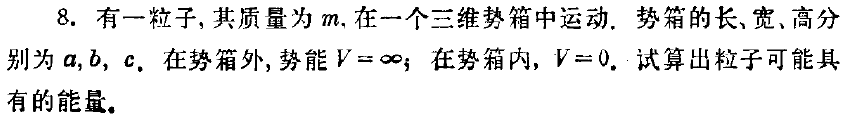
\includegraphics[width=\linewidth]{figures/8}
  \label{fig:}
\end{figure}

\begin{equation*}
  \begin{aligned}
    \dfrac{\partial^2 \Psi}{\partial x^2} + \dfrac{\partial^2 \Psi}{\partial y^2} + \dfrac{\partial^2 \Psi}{\partial z^2} + \dfrac{2 m }{\hbar^2} \left[ E - \left( V_x + V_y + V_Z \right) \right] \Psi = 0  
  \end{aligned}
\end{equation*}

\begin{equation*}
  V = \left\{
  \begin{aligned}
    & 0 \quad - a/2 < x < a/2, - b/2 < y < b/2, - c/2 < z < c/2 \\
    & \infty \quad \mathrm{others}
  \end{aligned}
  \right.
\end{equation*}



Let

\begin{equation*}
  \begin{aligned}
    \Psi \left( x, y, z \right) = X \left( x \right) Y \left( y \right) Z \left( z \right)
  \end{aligned}
\end{equation*}

Insert it into, we got

\begin{equation*}
  \begin{aligned}
    \left( \dfrac{1}{X} \dfrac{\md^2 X}{\md x^2} - \dfrac{2 m}{\hbar^2} V_x \right) + \left( \dfrac{1}{Y} \dfrac{\md^2 Y}{\md y^2} - \dfrac{2 m}{\hbar^2} V_y \right) + \left( \dfrac{1}{Z} \dfrac{\md^2 Z}{\md z^2} - \dfrac{2 m}{\hbar^2} V_z \right) + \dfrac{2 m E}{\hbar} = 0
  \end{aligned}
\end{equation*}

So we can separate the 3 variables

\begin{equation*}
  \left\{
  \begin{aligned}
    & \left( \dfrac{1}{X} \dfrac{\md^2 X}{\md x^2} - \dfrac{2 m}{\hbar^2} V_x \right) - \dfrac{2 m E_x}{\hbar} = 0 \\
    & \left( \dfrac{1}{Y} \dfrac{\md^2 Y}{\md y^2} - \dfrac{2 m}{\hbar^2} V_y \right) - \dfrac{2 m E_y}{\hbar} = 0 \\
    & \left( \dfrac{1}{Z} \dfrac{\md^2 Z}{\md z^2} - \dfrac{2 m}{\hbar^2} V_z \right) - \dfrac{2 m E_z}{\hbar} = 0
  \end{aligned}
  \right.
\end{equation*}

The solution is

\begin{equation*}
  \left\{
  \begin{aligned}
    & E_x = \dfrac{\pi^2 \hbar^2}{2 m a^2} n_x^2 \\ 
    & E_y = \dfrac{\pi^2 \hbar^2}{2 m b^2} n_y^2 \\ 
    & E_z = \dfrac{\pi^2 \hbar^2}{2 m c^2} n_z^2 \\ 
  \end{aligned}
  \right.
\end{equation*}

And the energy that the particle may have in total is

\begin{equation*}
  \begin{aligned}
    E = E_x + E_y + E_z = \dfrac{\pi^2 \hbar^2}{2 m} \left( \dfrac{n_x^2}{a^2} + \dfrac{n_y^2}{b^2} + \dfrac{n_z^2}{c^2} \right)
  \end{aligned}
\end{equation*}




\end{document}